\chapter{Identità digitale}

\section{Analisi dei requisiti}
Come da requisiti, l’obbiettivo principale di BLINC è quello di creare un portadocumenti digitale
i cui documenti inseriti rimangono sotto il controllo del proprietario.

Questo requisito introduce il concetto di \textbf{sovranità del dato} (o self-sovereign identity), ovvero il totale
controllo della propria identità digitale senza dover dipendere da terzi come Facebook o SPID per la Pubblica Amministrazione.

La self-sovereign identity è soltanto l’ultima di una serie di evoluzioni che la gestione dell’identità digitale
ha subìto nel tempo: inizialmente si aveva il modello a silos, ovvero la creazione di credenziali diverse per ogni
servizio di cui un utente fruisce.

Successivamente si è passati ad un modello federato, nel quale le credenziali per un determinato servizio/sistema
vengono riconosciute ed accettate anche in altri sistemi. Esempi di questo modello applicato in generale sono
Facebook e Google Login, tramite i quali si può accedere ai siti/applicazioni che li supportano utilizzando le
proprie credenziali Facebook/Google, mentre SPID è un esempio di un’applicazione a livello di Pubblica Amministrazione 
di questo modello. 

La self-sovereign identity non sarebbe mai stata possibile con i tradizionali sistemi di Identity Providing
centralizzati, ma con l’avvento della blockchain si è finalmente potuto iniziare ad esplorare soluzioni di sovranità
del dato grazie soprattutto a due importanti proprietà: la \textbf{pseudonimizzazione} e la \textbf{decentralizzazione}.

La prima è fondamentale anche in ottica GDPR ed è data dall’intrinseca capacità della blockchain di mantenere 
riferimenti ad informazioni tramite il loro hash, la seconda è importante in quanto un 
identity provider basato su blockchain è sempre disponibile al contrario degli identity provider centralizzati che,
se non disponibili, impossibilitano l’accesso a servizi.
Alcune aziende stanno implementando soluzioni di self-sovereign identity, e per BLINC sono state esaminate e
valutate le seguenti:

\section{Elenco dei prodotti e delle tecnologie disponibili}

\begin{itemize}
  \item \textbf{uPort}:
  Sviluppato sotto l’egida di ConsenSys, uPort è un sistema per la self-sovereign identity basato su Ethereum. 

  \item \textbf{Civic}:

  Civic è una piattaforma composta da smart contract ed un token per lo scambio
  di valore basata su Rootstock, una side-chain di Bitcoin che permette l’esecuzione di smart contract.

  Civic fornisce una piattaforma sicura di self-sovereign identity accessibile dagli utenti tramite
  la loro app, che funge da wallet per l’identità.
  Civic ed i suoi identity partner possono fare una richiesta di credenziali all’utente, che può 
  accettare o respingere, tramite un codice QR.
  Nel sistema Civic i\emph{Validatori}, ovvero istituzioni finanziarie, entità governative e aziende che hanno la possibilità
  di validare l’identità di singoli o di altre aziende che prendono parte al sistema
  Civic come \emph{Utenti} tramite delle transazioni di approvazione sulla blockchain chiamate attestazioni.
  Una attestazione è in pratica l’hash di un’informazione dell’identità più metadati relativi ad essa
  utilizzabile dai \emph{Fornitori di servizi} per erogare servizi agli utenti abilitati. I fornitori di servizi possono
  acquistare le attestazioni ai validatori tramite smart contract pagando con i token del sistema Civic.

  \begin{figure}[!ht]
    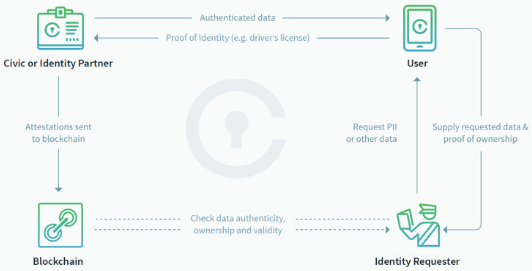
\includegraphics[scale=0.5]{civic}
    \caption{Diagramma di funzionamento di Civic.}
    \label{fig:civic}
  \end{figure}

  \item \textbf{SelfKey}:

  Sviluppato dalla SelfKey Foundation, SelfKey è un sistema basato su Blockchain Ethereum composto
  da un wallet personale per il possessore dell’identità, un marketplace di prodotti e servizi,
  un protocollo basato su JSON-LD ed un token per scambiare valore.
  L’identità dell’utente è salvata localmente sul suo smartphone sottoforma di wallet (coppia di chiavi),
  al quale vengono associate delle dichiarazioni sugli attributi dell’utente (data di nascita, nome, lavoro…) 
  che possono essere verificate da terzi (banche, organizzazione…)
  in modo da poter accedere a determinati servizi. Con questo metodo si riduce
  la quantità di dati condivisi alle terze parti allo stretto indispensabile.
  
  \begin{figure}[!ht]
    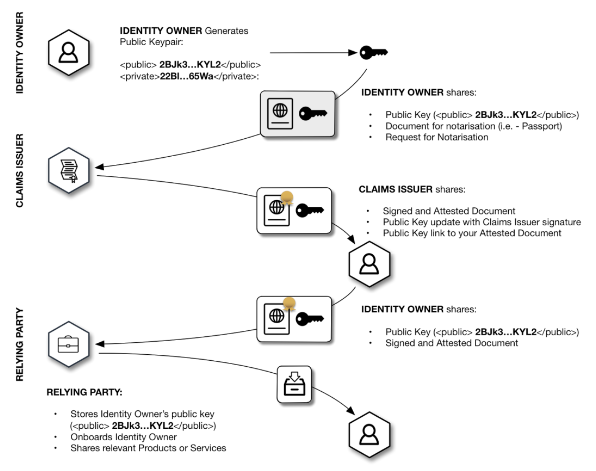
\includegraphics[width=\linewidth]{selfkey}
    \caption{Diagramma di funzionamento di SelfKey.}
    \label{fig:selfkey}
  \end{figure}
\end{itemize}

\section{Descrizione della tecnologia scelta e motivazione}

uPort è un insieme di protocolli, librerie e smart contract che creano uno strato interoperabile di identità,
che possono aggiungere, togliere e verificare attributi ed attestazioni a sé stesse ed alle altre identità.

Un’identità in uPort è formata da:

\begin{itemize}
  \item Un \textbf{MNID} (Multi Network IDentifier), che è un oggetto JSON codificato in base58 formato da un campo network, ovvero l’ID della chain Ethereum su cui si trova l’account
  (ad esempio 0x1 per la mainnet) e un campo address il cui valore è un indirizzo Ethereum.
  \item Una chiave privata necessaria per firmare transazioni da inviare alla blockchain.
  \item Una chiave pubblica inserita nel proprio DID Document (un oggetto JSON) salvato su IPFS e sullo smart contract Registry.
\end{itemize}

uPort prevede la gestione di dati sia off-chain che on-chain. 

\subsection{uPort on-chain: smart contract per l'identità}

Per quanto riguarda la parte on-chain uPort prevede un insieme di smart contract per la gestione delle identità che sono:

\begin{itemize}
  \item \texttt{Proxy}: uno per ogni identità, funge da rappresentante on-chain di essa. Ogni transazione che viene fatta
  sulla blockchain viene fatta dallo smart contract Proxy e non direttamente dal wallet dell’identità, permettendo
  di conseguenza di mantenere il possesso della propria identità digitale anche nel caso di smarrimento del 
  device su cui è installato il wallet uPort.

  \begin{lstlisting}[language=Solidity]
// Proxy.sol
pragma solidity 0.4.15;
import "./libs/Owned.sol";


contract Proxy is Owned {
    event Forwarded (address indexed destination, uint value, bytes data);
    event Received (address indexed sender, uint value);

    function () payable { Received(msg.sender, msg.value); }

    function forward(address destination, uint value, bytes data) public onlyOwner {
        require(executeCall(destination, value, data));
        Forwarded(destination, value, data);
    }

    // copied from GnosisSafe
    // https://github.com/gnosis/gnosis-safe-contracts/blob/master/contracts/GnosisSafe.sol
    function executeCall(address to, uint256 value, bytes data) internal returns (bool success) {
        assembly {
            success := call(gas, to, value, add(data, 0x20), mload(data), 0, 0)
        }
    }
}
  \end{lstlisting}
  \item \texttt{IdentityManager}: uno per chain, funge da Factory degli smart contract Proxy e ne tiene traccia,
  associando, oltre all’identità vera e propria associata al Proxy, altre identità fidate che permettono
  il recupero del possesso del proprio contract Proxy in caso di smarrimento del wallet.

  \begin{lstlisting}[language=Solidity]
// IdentityManager.sol
pragma solidity 0.4.15;
import "./Proxy.sol";


contract IdentityManager {
    uint adminTimeLock;
    uint userTimeLock;
    uint adminRate;

    event LogIdentityCreated(
        address indexed identity,
        address indexed creator,
        address owner,
        address indexed recoveryKey);

    event LogOwnerAdded(
        address indexed identity,
        address indexed owner,
        address instigator);

    event LogOwnerRemoved(
        address indexed identity,
        address indexed owner,
        address instigator);

    event LogRecoveryChanged(
        address indexed identity,
        address indexed recoveryKey,
        address instigator);

    event LogMigrationInitiated(
        address indexed identity,
        address indexed newIdManager,
        address instigator);

    event LogMigrationCanceled(
        address indexed identity,
        address indexed newIdManager,
        address instigator);

    event LogMigrationFinalized(
        address indexed identity,
        address indexed newIdManager,
        address instigator);

    mapping(address => mapping(address => uint)) owners;
    mapping(address => address) recoveryKeys;
    mapping(address => mapping(address => uint)) limiter;
    mapping(address => uint) public migrationInitiated;
    mapping(address => address) public migrationNewAddress;

    modifier onlyOwner(address identity) {
        require(isOwner(identity, msg.sender));
        _;
    }

    modifier onlyOlderOwner(address identity) {
        require(isOlderOwner(identity, msg.sender));
        _;
    }

    modifier onlyRecovery(address identity) {
        require(recoveryKeys[identity] == msg.sender);
        _;
    }

    modifier rateLimited(address identity) {
        require(limiter[identity][msg.sender] < (now - adminRate));
        limiter[identity][msg.sender] = now;
        _;
    }

    modifier validAddress(address addr) { //protects against some weird attacks
        require(addr != address(0));
        _;
    }

    /// @dev Contract constructor sets initial timelock limits
    /// @param _userTimeLock Time before new owner added by recovery can control proxy
    /// @param _adminTimeLock Time before new owner can add/remove owners
    /// @param _adminRate Time period used for rate limiting a given key for admin functionality
    function IdentityManager(uint _userTimeLock, uint _adminTimeLock, uint _adminRate) {
        require(_adminTimeLock >= _userTimeLock);
        adminTimeLock = _adminTimeLock;
        userTimeLock = _userTimeLock;
        adminRate = _adminRate;
    }

    /// @dev Creates a new proxy contract for an owner and recovery
    /// @param owner Key who can use this contract to control proxy. Given full power
    /// @param recoveryKey Key of recovery network or address from seed to recovery proxy
    /// Gas cost of 289,311
    function createIdentity(address owner, address recoveryKey) public validAddress(recoveryKey) {
        Proxy identity = new Proxy();
        owners[identity][owner] = now - adminTimeLock; // This is to ensure original owner has full power from day one
        recoveryKeys[identity] = recoveryKey;
        LogIdentityCreated(identity, msg.sender, owner,  recoveryKey);
    }

    /// @dev Creates a new proxy contract for an owner and recovery and allows an initial forward call which would be to set the registry in our case
    /// @param owner Key who can use this contract to control proxy. Given full power
    /// @param recoveryKey Key of recovery network or address from seed to recovery proxy
    /// @param destination Address of contract to be called after proxy is created
    /// @param data of function to be called at the destination contract
    function createIdentityWithCall(address owner, address recoveryKey, address destination, bytes data) public validAddress(recoveryKey) {
        Proxy identity = new Proxy();
        owners[identity][owner] = now - adminTimeLock; // This is to ensure original owner has full power from day one
        recoveryKeys[identity] = recoveryKey;
        LogIdentityCreated(identity, msg.sender, owner,  recoveryKey);
        identity.forward(destination, 0, data);
    }

    /// @dev Allows a user to transfer control of existing proxy to this contract. Must come through proxy
    /// @param owner Key who can use this contract to control proxy. Given full power
    /// @param recoveryKey Key of recovery network or address from seed to recovery proxy
    /// Note: User must change owner of proxy to this contract after calling this
    function registerIdentity(address owner, address recoveryKey) public validAddress(recoveryKey) {
        require(recoveryKeys[msg.sender] == 0); // Deny any funny business
        owners[msg.sender][owner] = now - adminTimeLock; // This is to ensure original owner has full power from day one
        recoveryKeys[msg.sender] = recoveryKey;
        LogIdentityCreated(msg.sender, msg.sender, owner, recoveryKey);
    }

    /// @dev Allows a user to forward a call through their proxy.
    function forwardTo(Proxy identity, address destination, uint value, bytes data) public onlyOwner(identity) {
        identity.forward(destination, value, data);
    }

    /// @dev Allows an olderOwner to add a new owner instantly
    function addOwner(Proxy identity, address newOwner) public onlyOlderOwner(identity) rateLimited(identity) {
        require(!isOwner(identity, newOwner));
        owners[identity][newOwner] = now - userTimeLock;
        LogOwnerAdded(identity, newOwner, msg.sender);
    }

    /// @dev Allows a recoveryKey to add a new owner with userTimeLock waiting time
    function addOwnerFromRecovery(Proxy identity, address newOwner) public onlyRecovery(identity) rateLimited(identity) {
        require(!isOwner(identity, newOwner));
        owners[identity][newOwner] = now;
        LogOwnerAdded(identity, newOwner, msg.sender);
    }

    /// @dev Allows an owner to remove another owner instantly
    function removeOwner(Proxy identity, address owner) public onlyOlderOwner(identity) rateLimited(identity) {
        // an owner should not be allowed to remove itself
        require(msg.sender != owner);
        delete owners[identity][owner];
        LogOwnerRemoved(identity, owner, msg.sender);
    }

    /// @dev Allows an owner to change the recoveryKey instantly
    function changeRecovery(Proxy identity, address recoveryKey) public
        onlyOlderOwner(identity)
        rateLimited(identity)
        validAddress(recoveryKey)
    {
        recoveryKeys[identity] = recoveryKey;
        LogRecoveryChanged(identity, recoveryKey, msg.sender);
    }

    /// @dev Allows an owner to begin process of transfering proxy to new IdentityManager
    function initiateMigration(Proxy identity, address newIdManager) public
        onlyOlderOwner(identity)
        validAddress(newIdManager)
    {
        migrationInitiated[identity] = now;
        migrationNewAddress[identity] = newIdManager;
        LogMigrationInitiated(identity, newIdManager, msg.sender);
    }

    /// @dev Allows an owner to cancel the process of transfering proxy to new IdentityManager
    function cancelMigration(Proxy identity) public onlyOwner(identity) {
        address canceledManager = migrationNewAddress[identity];
        delete migrationInitiated[identity];
        delete migrationNewAddress[identity];
        LogMigrationCanceled(identity, canceledManager, msg.sender);
    }

    /// @dev Allows an owner to finalize migration once adminTimeLock time has passed
    /// WARNING: before transfering to a new address, make sure this address is "ready to recieve" the proxy.
    /// Not doing so risks the proxy becoming stuck.
    function finalizeMigration(Proxy identity) public onlyOlderOwner(identity) {
        require(migrationInitiated[identity] != 0 && migrationInitiated[identity] + adminTimeLock < now);
        address newIdManager = migrationNewAddress[identity];
        delete migrationInitiated[identity];
        delete migrationNewAddress[identity];
        identity.transfer(newIdManager);
        delete recoveryKeys[identity];
        // We can only delete the owner that we know of. All other owners
        // needs to be removed before a call to this method.
        delete owners[identity][msg.sender];
        LogMigrationFinalized(identity, newIdManager, msg.sender);
    }

    function isOwner(address identity, address owner) public constant returns (bool) {
        return (owners[identity][owner] > 0 && (owners[identity][owner] + userTimeLock) <= now);
    }

    function isOlderOwner(address identity, address owner) public constant returns (bool) {
        return (owners[identity][owner] > 0 && (owners[identity][owner] + adminTimeLock) <= now);
    }

    function isRecovery(address identity, address recoveryKey) public constant returns (bool) {
        return recoveryKeys[identity] == recoveryKey;
    }
}
  \end{lstlisting}

  \item \textbf{UportRegistry}: uno per chain, serve per aggiungere attributi in forma chiave:valore alle identità,
  in particolare l’hash del DID Document caricato su IPFS.
  
  \begin{lstlisting}[language=Solidity]
//UportRegistry.sol
pragma solidity 0.4.8;

contract UportRegistry{
  uint public version;
  address public previousPublishedVersion;
  mapping(bytes32 => mapping(address => mapping(address => bytes32))) public registry;

  function UportRegistry(address _previousPublishedVersion) {
    version = 3;
    previousPublishedVersion = _previousPublishedVersion;
  }

  event Set(
    bytes32 indexed registrationIdentifier,
    address indexed issuer,
    address indexed subject,
    uint updatedAt);

  //create or update
  function set(bytes32 registrationIdentifier, address subject, bytes32 value){
      Set(registrationIdentifier, msg.sender, subject, now);
      registry[registrationIdentifier][msg.sender][subject] = value;
  }

  function get(bytes32 registrationIdentifier, address issuer, address subject) constant returns(bytes32){
      return registry[registrationIdentifier][issuer][subject];
  }
}
  \end{lstlisting}

  \item \texttt{EthereumClaimsRegistry}: uno per chain, serve per aggiungere dichiarazioni ed attestazioni alle identità.
  
  \begin{lstlisting}[language=Solidity]
//EthereumClaimsRegistry.sol
pragma solidity 0.4.19;


/// @title Ethereum Claims Registry - A repository storing claims issued
///        from any Ethereum account to any other Ethereum account.
contract EthereumClaimsRegistry {

    mapping(address => mapping(address => mapping(bytes32 => bytes32))) public registry;

    event ClaimSet(
        address indexed issuer,
        address indexed subject,
        bytes32 indexed key,
        bytes32 value,
        uint updatedAt);

    event ClaimRemoved(
        address indexed issuer,
        address indexed subject,
        bytes32 indexed key,
        uint removedAt);

    /// @dev Create or update a claim
    /// @param subject The address the claim is being issued to
    /// @param key The key used to identify the claim
    /// @param value The data associated with the claim
    function setClaim(address subject, bytes32 key, bytes32 value) public {
        registry[msg.sender][subject][key] = value;
        ClaimSet(msg.sender, subject, key, value, now);
    }

    /// @dev Create or update a claim about yourself
    /// @param key The key used to identify the claim
    /// @param value The data associated with the claim
    function setSelfClaim(bytes32 key, bytes32 value) public {
        setClaim(msg.sender, key, value);
    }

    /// @dev Allows to retrieve claims from other contracts as well as other off-chain interfaces
    /// @param issuer The address of the issuer of the claim
    /// @param subject The address to which the claim was issued to
    /// @param key The key used to identify the claim
    function getClaim(address issuer, address subject, bytes32 key) public constant returns(bytes32) {
        return registry[issuer][subject][key];
    }

    /// @dev Allows to remove a claims from the registry.
    ///      This can only be done by the issuer or the subject of the claim.
    /// @param issuer The address of the issuer of the claim
    /// @param subject The address to which the claim was issued to
    /// @param key The key used to identify the claim
    function removeClaim(address issuer, address subject, bytes32 key) public {
        require(msg.sender == issuer || msg.sender == subject);
        require(registry[issuer][subject][key] != 0);
        delete registry[issuer][subject][key];
        ClaimRemoved(msg.sender, subject, key, now);
    }
}
  \end{lstlisting}
\end{itemize}

\subsection{uPort off-chain: JWT per lo scambio di informazioni}

Per quanto riguarda invece le interazioni off-chain uPort utilizza JWT (JSON Web Token)
firmati, che possono essere utilizzati per:
\begin{itemize}
  \item Ricevere/fare richieste di condivisione di credenziali da/ad altre identità uPort
  \item Inviare/ricevere attestazioni a/da altre identità uPort
\end{itemize}

\subsection{JSON Web Token}

I \textbf{JWT} sono una maniera standardizzata dalla RFC per scambiare informazioni
tra parti sotto forma di oggetto JSON firmato ed eventualmente criptato.

Sono utilizzati principalmente in due ambiti:
\begin{enumerate}
  \item \textbf{Autorizzazione}: una volta che un utente ha acceduto ad un sito/servizio,
  un JWT viene aggiunto ad ogni richiesta successiva per consentire
  l’accesso a risorse protette (API, ad esempio).
  \item \textbf{Scambio di informazioni}: ambito d’interesse per uPort,
  un JWT è particolarmente indicato per scambiare informazioni per due motivi:
  è un formato di dimensioni ridotte adatto ad essere aggiunto ad un URL
  ed essendo un oggetto JSON firmato si ha la sicurezza che le informazioni ricevute
  siano quelle inviate inizialmente e che non siano state modificate nel frattempo.
\end{enumerate}

\subsubsection{Formato di un JWT}

Un esempio di JWT codificato è questo:

\begin{figure}[!ht]
    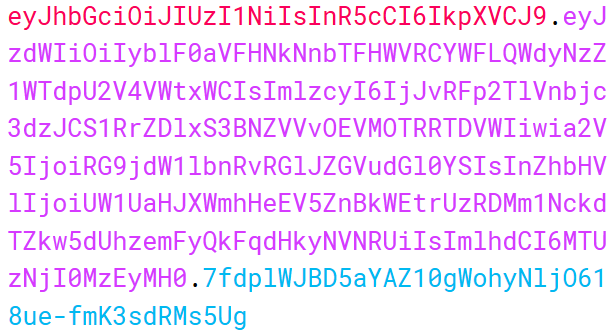
\includegraphics[width=\linewidth]{jwt}
    \caption{Esempio di JWT codificato.}
    \label{fig:jwt}
\end{figure}

Come si vede un JWT è diviso in tre parti separate dai punti:

\begin{itemize}
    \definecolor{headerColor}{RGB}{251, 1, 91}
    \definecolor{payloadColor}{RGB}{214, 58, 255}
    \definecolor{signatureColor}{RGB}{0, 185, 241}
    \item {\color{headerColor} Header}: un oggetto JSON codificato in Base64
    composto dal tipo di token (JWT) e dall'algoritmo di hash 
    usato, nel caso in foto HMAC SHA256
    \item {\color{payloadColor} Payload}: un oggetto JSON codificato in base64
    che contiene le dichiarazioni
    che vengono fatte su un soggetto, nel caso di uPort su un'identità, e le informazioni
    su quella dichiarazione, ad esempio:

    \begin{lstlisting}
{
    "key": "CartaDiIdentita",
    "value": "hashIPFSdellacartadiidentita"
}
    \end{lstlisting}
    \item {\color{signatureColor} Signature}: un hash dell'Header codificato in base64,
    un ".", Payload codificato in base64 e un secret.
\end{itemize}

Come si deduce dall'immagine sopra, i JWT permettono di inviare 
molte informazioni in un formato molto ristretto, adatto quindi ad essere incluso in un
URL di una richiesta HTTP, ad esempio. 

uPort utilizza i JWT esattamente in questo modo: si inviano ad un unico endpoint
\texttt{https://id.uport.me/req/[JWT]},
il quale si occuperà poi di decodificare e, in base al contenuto del payload,
agire di conseguenza richiedendo informazioni, aggiungendo
dichiarazioni o richiedendo di firmare transazioni all'utente specificato nel JWT. 

\subsection{uPort e la sovranità del dato}

uPort, come tutte le soluzioni di self-sovereign identity, inverte totalmente
il paradigma dell’identità online:
se prima erano i siti web e servizi su cui ci si registrava ad avere sotto controllo
tutte le nostre informazioni, avendo quindi la possibilità di utilizzarle per scopi pubblicitari od altro,
con uPort l’identità e le informazioni associate ad essa sono totalmente sotto il controllo del
proprietario dell’identità e sono le terze parti a dover richiedere le informazioni necessarie all’utente,
che di conseguenza ha anche un maggiore controllo su quali e quante informazioni fornisce.

Questo processo di rilascio di informazioni personali a terzi
in uPort si chiama \textbf{Selective Disclosure Flow}, e segue questo flusso:

\newpage

\begin{figure}[!ht]
    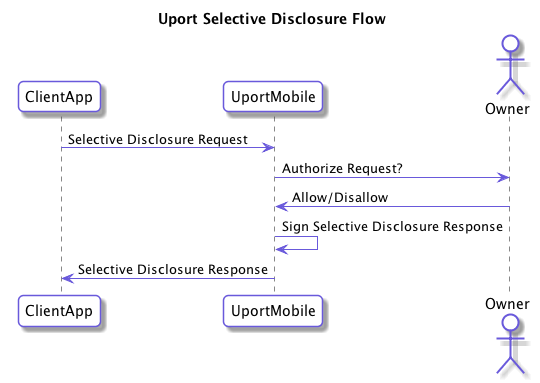
\includegraphics[width=\linewidth]{selectivedisclosure}
    \caption{Diagramma di sequenza per la richiesta di informazioni ad un utente uPort.}
    \label{fig:selectivedisclosure}
\end{figure}

La \textbf{Selective Disclosure Request} fatta dal servizio che richiede le credenziali
all’utente è un JWT che segue uno schema ben formato inviato ad un
opportuno endpoint gestito da uPort. 

\begin{table}[htbp]
    \centering
    \caption{Campi di una Selective Disclosure Request}
      \begin{tabular}{p{6.165em}p{19.89em}p{6.335em}}
      \toprule
      \textbf{Nome} & \textbf{Descrizione} & \textbf{Obbligatorio} \\
      \midrule
      \texttt{type} & Deve avere valore shareReq & Sì \\
      \midrule
      \texttt{iss} & Il MNID dell’identità firmataria & Sì \\
      \midrule
      \texttt{iat} & Il momento del rilascio & Sì \\
      \midrule
      \texttt{exp} & Momento di scadenza del JWT & No \\
      \midrule
      \texttt{callback} & URL di callback per restituire la risposta ad una richiesta & No \\
      \midrule
      \texttt{net} & Id della rete della chain Ethereum dell’Identità. Es. 0x4 per rinkeby & No \\
      \midrule
      \texttt{act} & Tipo dell’account Ethereum: \newline{}- General: scelta dell’utente (default)\newline{}- Segregated: un account basato su uno smart contract unico sarà creato per l’app richiedente\newline{}- Keypair: un account basato su una coppia di chiavi unica sarà creato per l’app richiedente\newline{}- Devicekey: richiede una nuova device key per un account su chain privata\newline{}- None: non viene restituito nessun account & No \\
      \midrule
      \texttt{requested} & Le attestazioni autofirmate da un utente. Vettore di tipi di attestazioni\newline{} per attestazioni autofirmate. Ad es: [“name, “email”] & No \\
      \midrule
      \texttt{verified} & Le attestazioni verificate richieste da un utente. Vettore di tipi di attestazioni per attestazioni autofirmate. Es: [“name”, “email”] & No \\
      \midrule
      \texttt{permissions} & Un vettore di permessi richiesti. Al momento sono solo supportate le notifications & No \\
      \midrule
      \texttt{boxPub} & Chiave pubblica del'identità richiedente, usata per criptare i messaggi inviati all'URL di callback & No \\
      \midrule
      \newpage
      \texttt{issc} & Le dichiarazioni auto firmate dal \texttt{iss} di questo messaggio, sia come oggetto di tipi di dichiarazioni
      per le dichiarazioni autofirmate oppure l'hash IPFS dell'oggetto equivalente. & No \\
      \midrule
      \texttt{vc} & Un vettore di dichiarazioni verificate (JWT) o l'hash IPFS dell'oggetto equivalente riguardanti
      il \texttt{iss} del messaggio  & No \\
      \bottomrule
      \end{tabular}%
    \label{tab:selectivedisclosurerequest}%
  \end{table}%

Una volta che la richiesta è arrivata al server
Chasqui (che gestisce lo scambio di JWT tra app uPort e normali web app o DApp)
la web app/DApp fa polling sul server fino a quando l’utente non approva o nega
l’accesso alle informazioni richieste: in caso di approvazione la web app/DApp ha
finalmente accesso alle informazioni richieste.

Molto spesso, come nel caso di BLINC, le informazioni vengono richieste per poi essere
attestate, ad esempio un servizio di e-ticketing potrebbe
richiedere nome e cognome dell’acquirente per attestare che
quell’identità ha effettivamente acquistato un biglietto. Per questo motivo
in congiunzione al flusso di richiesta di informazioni uPort prevede il
\textbf{Send Verification Flow}, ovvero il processo di attestazione di attributi
e credenziali dell’identità.

\newpage

\begin{figure}[!ht]
    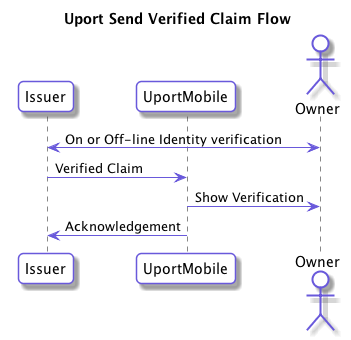
\includegraphics{verifiedclaim}
    \caption{Diagramma di sequenza per l'aggiunta di dichiarazioni su un'identità uPort.}
    \label{fig:verifiedclaim}
\end{figure}

Il Verified Claim creato dall’issuer (che è l’identità uPort che ha creato l’attestazione)
è un JWT che segue uno schema ben formato inviato allo stesso server Chasqui citato
in precedenza e segue un flusso molto simile a quello della richiesta di credenziali.

\subsection{Perché è stato scelto uPort?}

Tra le tre opzioni esplorate si è deciso di adottare uPort per i seguenti motivi:

\begin{itemize}
    \item Basato su piattaforma Ethereum: per motivi di facilità di sviluppo e di deploy di blockchain privata è stato scelto
    Ethereum per BLINC, quindi Civic, basato su Rootstock, è stato scartato per questo motivo.
    \item Semplice e interoperabile con altri smart contract: uPort è un semplice layer di identità basato su 
    smart contract Ethereum senza servizi o token aggiuntivi, motivo per cui è stato preferito a SelfKey.
    \item Grado di maturità: tra le tre opzioni esplorate, uPort è quello in stato più avanzato di sviluppo e ha il miglior supporto
    sia dal team di sviluppo che dalla community.
\end{itemize}

\section{Integrazione nel progetto BLINC}

All’interno del progetto uPort è stato utilizzato per la gestione di dichiarazioni
ed endorsement sui migranti e la creazione di uPort Identity associate ad essi.

\subsection{Gestione di dichiarazioni ed endorsement}
Per quanto riguarda questo caso d’uso di BLINC ci si
riferisce a questo flusso di interazione:

\begin{figure}[!ht]
    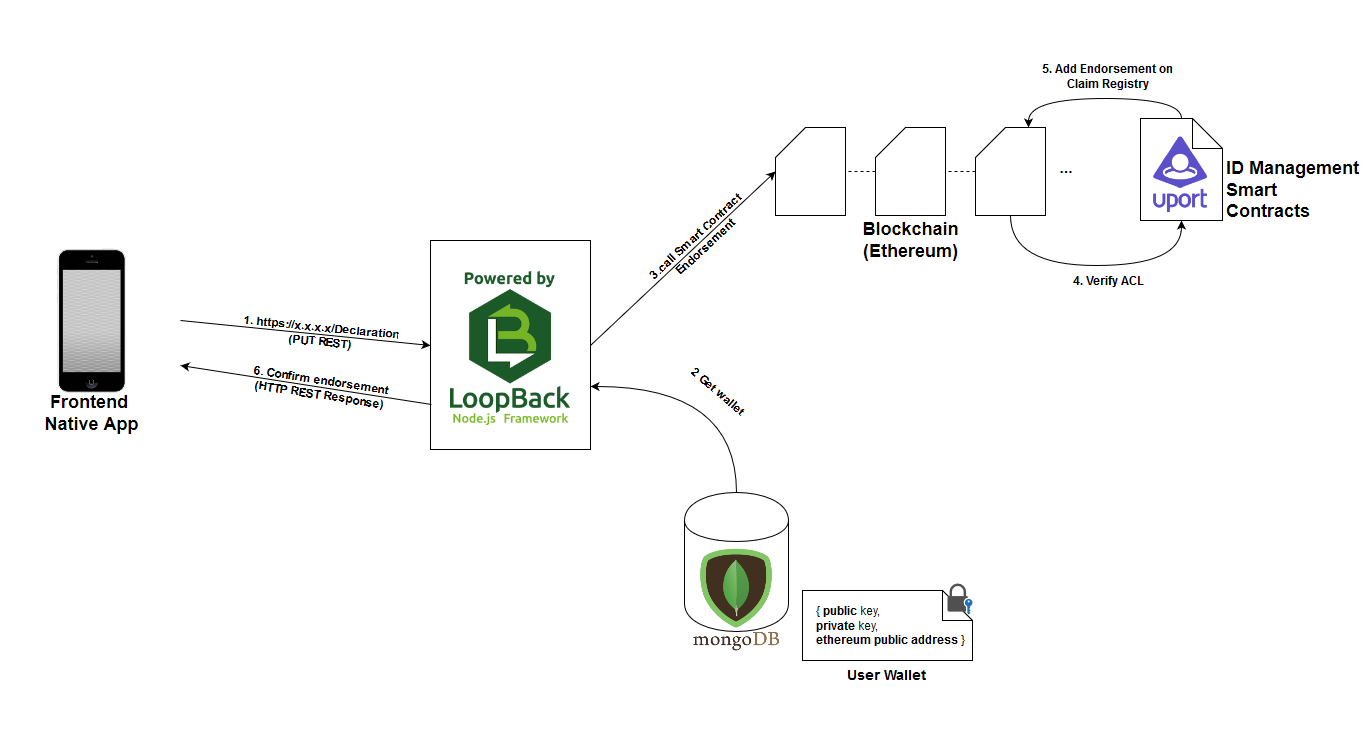
\includegraphics[width=\linewidth]{adddeclarations}
    \caption{Flusso di gestione delle dichiarazioni sull'utente.}
    \label{fig:adddeclarations}
  \end{figure}

Alla rispettiva chiamata API il backend di BLINC va a recuperare dal database
il wallet associato al migrante che si è autenticato e firma una transazione
che ha come destinatario lo smart contract ethereum-claims-registry, che permette
di associare delle dichiarazioni da parte di un indirizzo Ethereum 
verso un altro in forma chiave:valore.

\textbf{Implementazione}

\begin{lstlisting}[language=JavaScript]
/**
* Gets all the declaration made and returns them.
* @param {string} id the id of the owner of the declarations.
*
* @returns {Array} declarations an array of declarations.
*/
Declaration.getAllDeclarations = (id, cb) => {
    Declaration.app.models.migrant.findOne(
    { where: { id } },
    async (err, instance) => {
        if (err) cb(err, null);
        const uportIdentity = initialize(instance);
        const declarations = await uportIdentity.getAllAttestations();
        cb(null, declarations);
    }
    );
};

/**
* Adds a declaration for a specific issuer
* @param {string} issuer the id of the owner of the declarations.
* @param {string} subject the subject of the declaration
* @param {string} key
* @param {string} value the value of the declaration itself
*
* @returns {Object} response the added declaration.
*/
Declaration.addDeclaration = (issuer, subject, key, value, cb) => {
    let issuerUportIdentity, signer, credentials, declaration, response;

    Declaration.app.models.migrant.findOne(
    { where: { id: issuer } },
    async (err, instance) => {
        if (err) cb(err, null);

        try {
        issuerUportIdentity = initialize(instance);

        // Gets the SimpleSigner object with the private key of the user, which is needed to sign transactions
        signer = SimpleSigner(issuerUportIdentity.deviceKeys.privateKey);

        // Instantiates the Credentials class, a uPort class which simplifies the creation of signed attestation JWTs
        credentials = new Credentials({
            address: issuerUportIdentity.mnid,
            signer: signer,
            networks: {
            [issuerUportIdentity.network.id]: {
                ...issuerUportIdentity.network
            }
            }
        });

        // The attest function creates a signed attestation JWT
        declaration = await credentials.attest({
            sub: subject,
            claim: { [key]: value }
        });

        // The consume function is a UPortClient function which parses uPort uris and relays them to the responsible functions
        response = await issuerUportIdentity.consume(
            `me.uport:add?attestations=${declaration}`
        );

        cb(null, response);
        } catch (error) {
        cb(error, null);
        }
    }
    );
};
\end{lstlisting}

\newpage

\subsection{Creazione di uPort Identity}

Si segue questo flusso ogni volta che un nuovo utente si iscrive alla piattaforma:

\begin{figure}[!ht]
    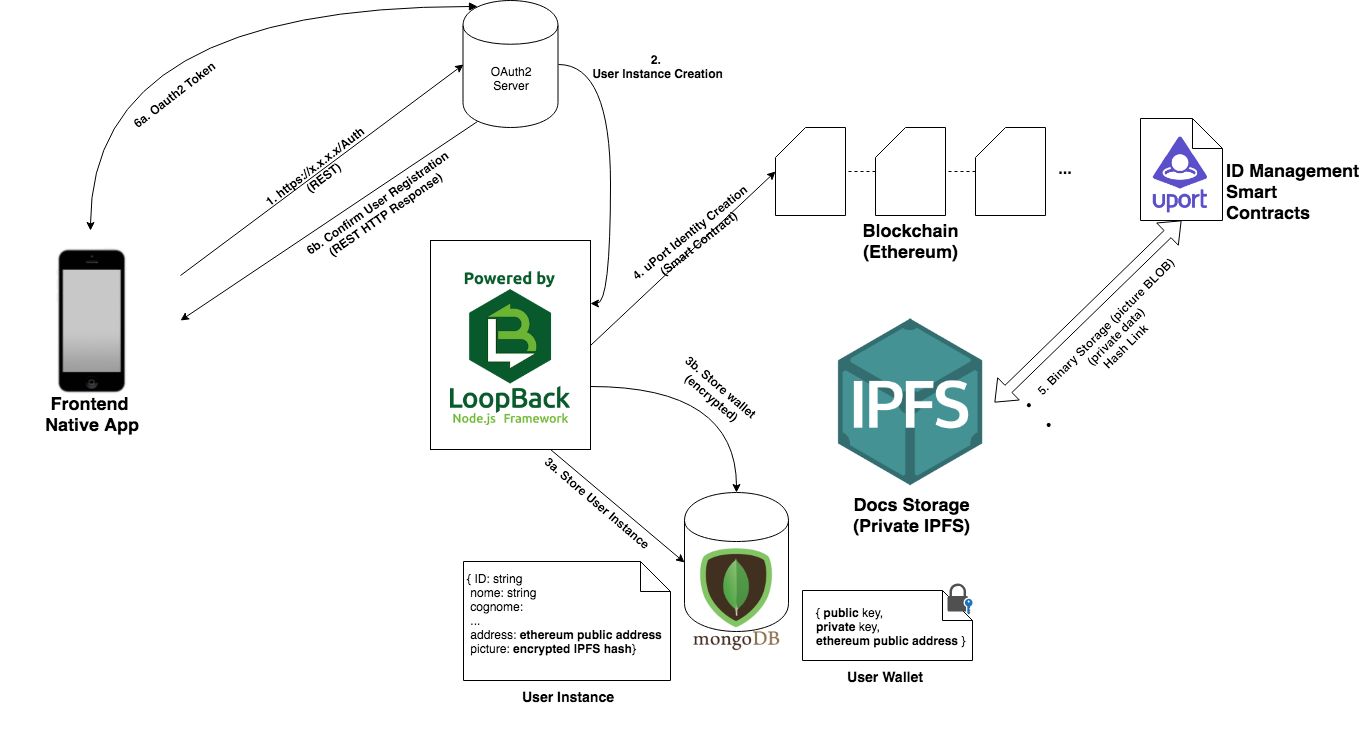
\includegraphics[width=\linewidth]{createidentities}
    \caption{Flusso di creazione di identità.}
    \label{fig:createidentities}
\end{figure}

Durante la registrazione viene istanziato sulla blockchain Ethereum privata 
lo smart contract Proxy associato all’utente e vengono salvate su database le credenziali
dell’utente (nome, cognome…) e gli si associa un wallet che viene poi criptato. A questo punto
ad ogni login dell’utente viene deserializzata l’identità uPort
ad esso associata ed il wallet, in modo da poter interagire con la blockchain.

\textbf{Implementazione}

\begin{lstlisting}[language=JavaScript]
/**
* creates a new migrant instance in uPort and in mongoDB.
* input params are personal info of the user.
* @param {String} name
* @param {String} familyName
* @param {string} phoneNumber
* @param {String} email
* @param {String} password
*
* @returns {Object} the migrant created instance
*/
Migrant.addMigrant = (name, familyName, phoneNumber, email, password, cb) => {
    Migrant.app.dataSources.BlincTestDB.autoupdate('migrant', async err => {
    if (err) throw err;

    let migrantID;

    const info = {
        name,
        familyName,
        phoneNumber,
        email,
        password
    };

    try {
        migrantID = await createUportId(info);
        migrantID = await initializeUportId(migrantID);
    } catch (error) {
        throw error;
    }

    migrantID = {
        id: migrantID.id,
        info: migrantID.info,
        deviceKeys: migrantID.deviceKeys,
        recoveryKeys: migrantID.recoveryKeys,
        mnid: migrantID.mnid,
        initialized: migrantID.initialized
    };

    Migrant.app.models.migrant.create([migrantID], function(err, migrant) {
        if (err) {
        cb(err, null);
        }
    });

    cb(null, migrantID);
    });
};

/**
* Gets a migrant from the datasource
* @param {String} email
* @param {String} password
*
* @returns {Object} the migrant instance
*/
Migrant.getMigrant = (email, password, cb) => {
    Migrant.app.models.migrant.findOne(
    { where: { 'info.email': email, 'info.password': password } },
    (err, instance) => {
        if (err) cb(err, null);

        cb(null, instance);
    }
    );
};
\end{lstlisting}

Le funzioni \texttt{createUportId} e \texttt{initializeUportId} fanno parte di una libreria scritta da me che funge da middleware tra
la business logic raggiungibile tramite chiamate API e la libreria \texttt{uport-js-client} (modificata ampiamente per i requisiti di BLINC),
che simula il funzionamento dei protocolli uPort. Qui il codice delle due funzioni:

\begin{lstlisting}[language=JavaScript]
/**
 * creates a UportClient instance.
 * @param {Object} info personal info of the user.
 *
 * @returns {Promise<UPortClient>} the promise to have a UPortClient with specified infos.
 */
const createUportId = (info = {}) => {
  return new Promise(async (resolve, reject) => {
    try {
      const uportClient = new UPortClient(config, { info });
      
      // Creates a keypair for the uPort client
      uportClient.initKeys();

      const accounts = await web3.eth.getAccounts();

      // Gets the first Ethereum account in the private blockchain which is the one who is mining hence
      // the one with funds  
      const miner = accounts[0];

      const fundTx = {
        from: miner,
        to: uportClient.deviceKeys.address,
        value: 0.2 * 1.0e18
      };

      // Sends transaction to fund the uPort client in order to deploy uPort contracts later
      await web3.eth.sendTransaction(fundTx);

      console.log('Funded identity');

      resolve(uportClient);
    } catch (e) {
      reject(e);
    }
  });
};
\end{lstlisting}

\begin{lstlisting}[language=JavaScript]
/**
* Initializes a UportClient instance, meaning that it will deploy uPort IdentityManager contract, save the DID Document on IPFS and save it on Registry contract.
* @param {UPortClient} uportClient an instance of UPortClient.
* @param {Object} appDDO facultative object with additional info in UPortClient is an instance of a uPort application
*
* @returns {Promise<UPortClient>} the promise to have a initialized UPortClient.
*/
const initializeUportId = (uportClient, appDDO = {}) => {
    return new Promise(async (resolve, reject) => {
    if (uportClient) {
        try {
            await uportClient.initializeIdentity(appDDO);
            resolve(uportClient);
        } catch (error) {
            reject(error);
        }
    } else reject('An uPort ID must be created!');
    });
};
\end{lstlisting}

La libreria \texttt{uport-js-client} mette a disposizione una classe

\texttt{UPortClient} così fatta:

\begin{lstlisting}[language=JavaScript]
class UPortClient {
    constructor(config = {}, initState = {}) {
        this.responseHandler = configResponseHandler(config.responseHandler);

        // Object that contains user's info if passed to the constructor, else empty object
        this.info = initState.info || {};

        // Keypair of the user necessary to sign transactions
        this.deviceKeys = config.deviceKeys;

        // Keypair of another identity, used to recover user's identity (Not used in BLINC as for now Identities are saved on a DB)
        this.recoveryKeys = config.recoveryKeys;

        /* Object with this form:
         *  network: {
         *   id: "0x456719", this is the id of the private blockchain deployed for BLINC
         *   rpcUrl: "http://10.83.0.11:8545", this is the endpoint we connect to in order to communicate with the blockchain via EthJS, a JavaScript library
         *   claimsRegistry: "0xa7b3058152165c72a4dd7c4812c5964f1c26f00d", this is the address of the EthereumClaimsRegistry contract on BLINC's private chain
         *   registry: "0xdb571079af66edbb1a56d22809584d39c20001d9", this is the address of the UportRegistry contract on BLINC's private chain
         *   identityManager: "0xff37a57b8d373518abe222db1077ed9a968a5fdf", this is the address of the IdentityManager contract on BLINC's private chain
         *   storage: "0x7e27e8f3aa4bda26502c38ccd28a4838aeca7966", this is the address of the smart contract that stores the IPFS hashes of user's documents
         *  },
         */
        this.network = config.network
        ? configNetwork(config.network)
        : configNetwork(networkConfig.network); // have some default connect/setup testrpc
    
        if (this.network) {
            // Crates an instance of the IPFS class, which allows us to communicate with the IPFS node specified in the configuration
            this.ipfs = new IPFS(networkConfig.ipfsConfig);
        
            this.registryNetwork = {
                [this.network.id]: {
                    registry: this.network.registry,
                    rpcUrl: this.network.rpcUrl
                }
            }
        };
    
        const registry = new UportLite({
            networks: this.registryNetwork
        });

        // Function that uses the UportLite library
        this.registry = address =>
            new Promise((resolve, reject) => {
                registry(address, (error, profile) => {
                    if (error) return reject(error);
        
                    resolve(profile);
                });
        });
    
        this.verifyJWT = jwt => verifyJWT({ registry: this.registry, address: this.mnid }, jwt);

        // Sets the HttpProvider, necessary object for EthJS library in order 
        // to interact with the Ethereum blockchain
        this.provider = config.provider || new HttpProvider(this.network.rpcUrl);

        // Creates the EthJS object with the just created HttpProvider as a parameter
        this.ethjs = this.provider ? new EthJS(this.provider) : null;

        // Sets addresses of contracts passed in the configuration object
        this.claimsRegistryAddress = this.network.claimsRegistry;
        this.registryAddress = this.network.registry;
        this.identityManagerAddress = this.network.identityManager;

        // Necessary to do some actions, if identity is recreated from MongoDB config.initialized has a value,
        // else identity is initialized later
        this.initialized = config.initialized || false;
    
        this.consume = this.consume.bind(this);
    }
}
\end{lstlisting}

Questo è il codice per inizializzare una identità uPort ed è richiamato dalla funzione da me creata \texttt{initializeUportId}

\begin{lstlisting}[language=JavaScript]
initializeIdentity(initDdo) {
    if (!this.network)
        return Promise.reject(new Error('No network configured'));

    const IdentityManagerAddress = this.identityManagerAddress;

    // Creates an object contract with a specific ABI 
    // (Application Binary Interface, a low level API-like for contracts, 
    // written in JSON as result of contract compilation)
    // and at a specific address for the IdentityManager contract
    const IdentityManager = Contract(IdentityManagerArtifact.abi).at(
        IdentityManagerAddress
    );

    // Creates keypair and an ethereum address for the user and for recovery
    this.initKeys();

    // Calls contract function to create an Identity
    const uri = IdentityManager.createIdentity(
        this.deviceKeys.address,
        this.recoveryKeys.address
    );

    // The consume function is a uport-js-client function which, given a URI which conforms to the uPort Protocol specs,
    // parses it and, basing on the given URI format, sends a tx, adds an attestation or requests credentials.
    return this.consume(uri)
    .then(this.getReceipt.bind(this))
    .then(receipt => {
        const log = receipt.logs[0];

        const createEventAbi = IdentityManager.abi.filter(
            obj => obj.type === 'event' && obj.name === 'IdentityCreated'
        )[0];

        // Gets the Proxy contract address for the identity from
        // the event emitted by the createIdentity function
        this.id = decodeEvent(createEventAbi, log.data, log.topics).identity;

        // Creates the MNID for the identity, which is the base58 encoding of the network id and the identity Proxy address
        this.mnid = mnid.encode({ network: this.network.id, address: this.id });
        this.initTransactionSigner(IdentityManagerAddress);

        const baseDdo = {
            '@context': 'http://schema.org',
            '@type': 'Person',
            publicKey: this.deviceKeys.publicKey
        };

        const ddo = Object.assign(baseDdo, initDdo);

        // The code for the writeDDO is below, at a high level it uploads the ddo object to IPFS
        // and adds it to the Registry smart contract
        return this.writeDDO(ddo);
    })
    .then(this.ethjs.getTransactionReceipt.bind(this.ethjs))
    .then(receipt => {
        
        this.initialized = true;
        return;
    });
}

writeDDO(newDdo) {
    // Creates an object contract with a specific ABI 
    // and at a specific address for the Registry contract
    const Registry = Contract(RegistryArtifact.abi).at(this.network.registry);
    return this.getDDO()
      .then(ddo => {
        // If the Identity Document already exists it doesn't overwrite with the given one,
        // otherwise it adds to IPFS the newDdo
        ddo = Object.assign(ddo || {}, newDdo);
        return new Promise((resolve, reject) => {
          this.ipfs.add(Buffer.from(JSON.stringify(ddo)), (err, result) => {
            if (err) reject(new Error(err));
            resolve(result);
          });
        });
      })
      .then(res => {
        const hash = res[0].hash;
        const hexhash = new Buffer(base58.decode(hash)).toString('hex');
        // Removes Qm from ipfs hash, which specifies length and hash
        const hashArg = `0x${hexhash.slice(4)}`;
        const key = 'uPortProfileIPFS1220';

        // Writes on the Registry contract the association between the Proxy contract address
        // for the identity and the IPFS hash of its Identity Document which contains its pubkey
        return Registry.set(key, this.id, hashArg);
      })
      .then(this.consume.bind(this));
}
\end{lstlisting}